\subsection{Discriminatore}

\subsubsection{Soglia}

Variamo la soglia del discriminatore collegato al fotodiodo e registriamo il corrispondente rate di eventi a \SI0{\degree} senza collimatori.
I valori di soglia riportati non hanno unità di misura perché sullo strumento sono solo presenti dei pallini e dei numeri interi. 
Non avendo trovato il manuale dello strumento, ci limitiamo a indicare la posizione del potenziometro.
Scopriamo (\autoref{fig:soglia}) che il valore della soglia è ininfluente fino a 0.7 e si ha una repentina variazione dopo questo valore.

\begin{figure}[h]
\centering
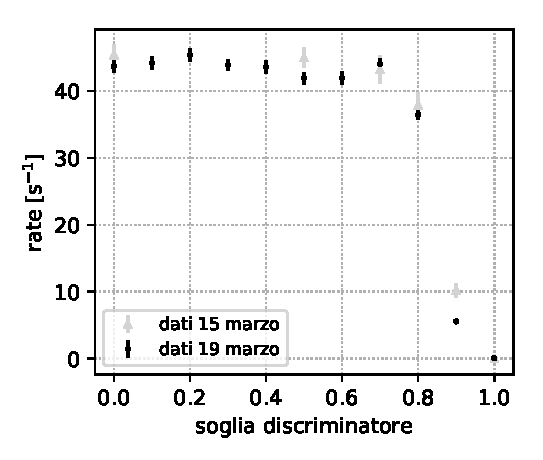
\includegraphics[width=30 em]{immagini/soglia}
\caption{Rate a 0$^{\circ}$ al variare della soglia del discriminatore con 2 set di dati.}
\label{fig:soglia}
\end{figure}

Per sapere se la soglia ha un effetto minore di quanto misurato dobbiamo aumentare la statistica. I rates misurati hanno (nel migliore dei casi) una precisione del 2\%.
Siccome il rate diminuisce di molto all'aumentare dell'angolo, le misure ad angoli maggiori avranno un'accuratezza minore. Quindi possiamo affermare che la soglia non avrà alcun effetto sulle misure di rate. 
Pertanto la teniamo a 0 per tutta l'esperienza.

\begin{table}[h]
\centering

\begin{tabular}{c|c}
soglia & rate [\si{s^{-1}}] \\
\hline
$ 0.0 $ & $ 45.4 \pm 1.5 $\\ 
$ 0.5 $ & $ 45.0 \pm 1.5 $\\ 
$ 0.7 $ & $ 43.2 \pm 2.1 $\\ 
$ 0.8 $ & $ 38 \pm 2 $\\ 
$ 0.9 $ & $ 10 \pm 1 $\\ 
$ 1.0 $ & $\;\; 0.05 \pm 0.05 $\\ 
\hline
$ 0.0 $ & $ 43.7 \pm 0.9 $\\ 
$ 0.1 $ & $ 44 \pm 1 $\\ 
$ 0.2 $ & $ 45 \pm 1 $\\ 
$ 0.3 $ & $ 43.9 \pm 0.8 $\\ 
$ 0.4 $ & $ 43.6 \pm 0.9 $\\ 
$ 0.5 $ & $ 41.9 \pm 0.9 $\\ 
$ 0.6 $ & $ 42.0 \pm 0.9 $\\ 
$ 0.7 $ & $ 44.0 \pm 0.9 $\\ 
$ 0.8 $ & $ 36.5 \pm 0.7 $\\ 
$ 0.9 $ & $ 5.6 \pm 0.2 $\\ 
$ 1.0 $ & $ 0.05 \pm 0.03 $\\ 

\end{tabular}

\caption{Valori presenti nel grafico di \autoref{fig:soglia}. La line orizzontale divide quelli del 15 marzo (in alto) da quelli del 19 marzo (in basso).}
\label{tab:soglia}
\end{table}

\subsubsection{Ritardo}

Guardando all'oscilloscopio i segnali da digitalizzare, ci siamo accorti che aumentare la soglia ritarda l'arrivo del segnale di trigger rendendo inutile la calibrazione dell'ADC ogni volta che la soglia viene modificata. Abbiamo quantificato questo effetto misurando il ritardo in funzione della soglia (\autoref{tab:rit}). 

